\chapter{用户程序与测试}

NimlothOS提供了丰富的用户程序集合,这些程序展示了操作系统的各种功能特性,从基础的进程管理到高级的调度算法测试。本章将按功能分类介绍这些用户程序的实现和用途。

\section{系统核心程序}

\subsection{initproc - 初始进程}

\texttt{initproc}是系统启动后运行的第一个用户进程,负责启动用户shell并管理僵尸进程的回收。
父进程通过fork创建子进程来运行shell,然后进入无限循环等待并回收所有退出的子进程,防止系统中出现僵尸进程。

\begin{lstlisting}[language=Rust]
fn main() -> i32 {
    if fork() == 0 {
        exec("user_shell\0", &[core::ptr::null::<u8>()]);
    } else {
        loop {
            let mut exit_code: i32 = 0;
            let pid = wait(&mut exit_code);
            if pid == -1 {
                yield_();
                continue;
            }
        }
    }
    0
}
\end{lstlisting}

\subsection{user\_shell - 用户命令行解释器}

\texttt{user\_shell}是一个命令行解释器,支持命令执行、管道操作和I/O重定向。

\begin{lstlisting}[language=Rust]
pub fn main() -> i32 {
    println!("{}", colored(logo, &format!("{}{}", C_BOLD, C_MAGENTA)));
    println_info("Rust User Shell - Type commands and press Enter.");
    let mut line: String = String::new();
    print_prompt();
    loop {
        let c = getchar();
        match c {
            LF | CR => {
                if !line.is_empty() {
                    let splited: Vec<_> = line.as_str().split('|').collect();
                    // 处理管道命令...
                }
                print_prompt();
            }
            // 处理其他输入...
        }
    }
}
\end{lstlisting}

Shell程序具有彩色界面显示、命令历史、管道支持和错误处理等功能。它能够解析用户输入的命令行,创建相应的进程,并通过管道连接多个命令。

\section{基础功能测试}

\subsection{hello\_world - 基础输出测试}

最简单的用户程序,验证用户态程序的基本运行能力。

\begin{lstlisting}[language=Rust]
pub fn main() -> i32 {
    println!("Hello world from user mode program!");
    0
}
\end{lstlisting}

\subsection{yield - 进程调度测试}

测试进程主动让出CPU的功能,验证调度器的基本工作机制。

\begin{lstlisting}[language=Rust]
pub fn main() -> i32 {
    println!("Hello, I am process {}.", pid());
    for i in 0..5 {
        yield_();
        println!("Back in process {}, iteration {}.", pid(), i);
    }
    println!("yield pass.");
    0
}
\end{lstlisting}

\subsection{cmdline\_args - 命令行参数测试}

验证命令行参数传递机制的正确性。

\begin{lstlisting}[language=Rust]
pub fn main(argc: usize, argv: &[&str]) -> i32 {
    println!("argc = {}", argc);
    for (i, arg) in argv.iter().enumerate() {
        println!("argv[{}] = {}", i, arg);
    }
    0
}
\end{lstlisting}

\section{进程管理测试}

\subsection{exit - 进程退出测试}

测试进程的fork、exit和wait机制,验证父子进程间的同步。

\begin{lstlisting}[language=Rust]
const MAGIC: i32 = -0x10384;

pub fn main() -> i32 {
    let pid = fork();
    if pid == 0 {
        println!("I am the child.");
        for _ in 0..7 { yield_(); }
        exit(MAGIC);
    } else {
        println!("I am parent, fork a child pid {}", pid);
    }
    let mut xstate: i32 = 0;
    assert!(waitpid(pid as usize, &mut xstate) == pid && xstate == MAGIC);
    0
}
\end{lstlisting}

\subsection{forktest系列 - 大量进程创建测试}

\textbf{forktest\_simple}测试基本的fork和wait功能:

\begin{lstlisting}[language=Rust]
pub fn main() -> i32 {
    assert_eq!(wait(&mut 0i32), -1); // 测试无子进程的wait
    let pid = fork();
    if pid == 0 {
        println!("hello child process!");
        100  // 子进程退出码
    } else {
        let mut exit_code: i32 = 0;
        assert_eq!(pid, wait(&mut exit_code));
        assert_eq!(exit_code, 100);
        0
    }
}
\end{lstlisting}

\textbf{forktest}创建30个子进程测试系统的进程管理能力:

\begin{lstlisting}[language=Rust]
const MAX_CHILD: usize = 30;

pub fn main() -> i32 {
    for i in 0..MAX_CHILD {
        let pid = fork();
        if pid == 0 {
            println!("I am child {}", i);
            exit(0);
        }
        assert!(pid > 0);
    }
    // 等待所有子进程结束
    for _ in 0..MAX_CHILD {
        if wait(&mut exit_code) <= 0 {
            panic!("wait stopped early");
        }
    }
    0
}
\end{lstlisting}

\textbf{forktree}创建二叉树形的进程结构,测试复杂的进程层次关系。

\subsection{matrix - 计算密集型测试}

通过矩阵乘法测试多进程并发计算能力。

\begin{lstlisting}[language=Rust]
fn work(times: isize) {
    let mut a: Arr = Default::default();
    let mut b: Arr = Default::default();
    let mut c: Arr = Default::default();
    
    for _ in 0..times {
        for i in 0..N {
            for j in 0..N {
                c[i][j] = 0;
                for k in 0..N {
                    c[i][j] = (c[i][j] + a[i][k] * b[k][j]) % P;
                }
            }
        }
    }
}
\end{lstlisting}

\section{调度器测试}

\subsection{MLFQ调度测试套件}

NimlothOS提供了完整的多级反馈队列(MLFQ)调度器测试程序。

\textbf{priority\_test}测试进程优先级降级机制:

\begin{lstlisting}[language=Rust]
fn cpu_bound_worker(worker_id: usize, work_amount: usize) {
    for i in 0..work_amount {
        let mut dummy = i;
        for _ in 0..1000 {
            dummy = (dummy * 1103515245 + 12345) & 0x7fffffff;
        }
        if completed_work % 10000 == 0 {
            println!("[Worker-{}] Progress: {}/{}",
                worker_id, completed_work, work_amount);
        }
    }
}
\end{lstlisting}

\textbf{io\_priority\_test}测试I/O密集型和CPU密集型进程的调度差异:

\begin{lstlisting}[language=Rust]
fn io_worker(process_id: usize) {
    while time() - start_time < 2000 {
        sleep(20);  // 模拟I/O操作
        // 做一些轻量计算
        let mut _result = 0;
        for i in 0..1000 {
            _result += i;
        }
    }
}
\end{lstlisting}

\textbf{mlfq\_demo}是一个综合演示程序,依次运行各个MLFQ测试来展示调度效果。

\section{文件系统测试}

\subsection{filetest\_simple - 基础文件操作}

测试文件的创建、写入和读取功能。

\begin{lstlisting}[language=Rust]
pub fn main() -> i32 {
    let test_str = "Hello, world!";
    let filea = "filea\0";
    // 写入测试
    let fd = open(filea, OpenFlags::CREATE | OpenFlags::WRONLY);
    write(fd, test_str.as_bytes());
    close(fd);
    // 读取测试
    let fd = open(filea, OpenFlags::RDONLY);
    let mut buffer = [0u8; 100];
    let read_len = read(fd, &mut buffer) as usize;
    close(fd);
    assert_eq!(test_str, core::str::from_utf8(&buffer[..read_len]).unwrap());
    0
}
\end{lstlisting}

\subsection{cat - 文件内容显示}

实现类似Unix的cat命令,读取并显示文件内容。

\begin{lstlisting}[language=Rust]
pub fn main(argc: usize, argv: &[&str]) -> i32 {
    assert!(argc == 2);
    let fd = open(argv[1], OpenFlags::RDONLY);
    let mut buf = [0u8; 256];
    loop {
        let size = read(fd, &mut buf) as usize;
        if size == 0 { break; }
        print!("{}", core::str::from_utf8(&buf[..size]).unwrap());
    }
    close(fd);
    0
}
\end{lstlisting}

\subsection{huge\_write - 大文件写入测试}

测试文件系统对大容量数据的处理能力和写入性能。

\begin{lstlisting}[language=Rust]
pub fn main() -> i32 {
    let mut buffer = [0u8; 1024]; // 1KiB
    for (i, ch) in buffer.iter_mut().enumerate() {
        *ch = i as u8;
    }
    let f = open("testf\0", OpenFlags::CREATE | OpenFlags::WRONLY);
    let start = time();
    let size_mb = 1usize;
    for _ in 0..1024 * size_mb {
        write(f, &buffer);
    }
    close(f);
    let time_ms = (time() - start) as usize;
    let speed_kbs = size_mb * 1000000 / time_ms;
    println!("{}MiB written, time cost = {}ms, write speed = {}KiB/s",
        size_mb, time_ms, speed_kbs);
    0
}
\end{lstlisting}

\section{管道通信测试}

\subsection{pipetest - 基础管道测试}

验证父子进程间通过管道进行通信的基本功能。

\begin{lstlisting}[language=Rust]
static STR: &str = "Hello, world!";

pub fn main() -> i32 {
    let mut pipe_fd = [0usize; 2];
    pipe(&mut pipe_fd);
    if fork() == 0 {
        // 子进程读取
        close(pipe_fd[1]);
        let mut buffer = [0u8; 32];
        let len_read = read(pipe_fd[0], &mut buffer) as usize;
        close(pipe_fd[0]);
        assert_eq!(core::str::from_utf8(&buffer[..len_read]).unwrap(), STR);
        0
    } else {
        // 父进程写入
        close(pipe_fd[0]);
        assert_eq!(write(pipe_fd[1], STR.as_bytes()), STR.len() as isize);
        close(pipe_fd[1]);
        wait(&mut child_exit_code);
        0
    }
}
\end{lstlisting}

\subsection{pipe\_large\_test - 大容量管道测试}

测试管道对大量数据传输的处理能力。

\begin{lstlisting}[language=Rust]
const LENGTH: usize = 3000;

pub fn main() -> i32 {
    let mut down_pipe_fd = [0usize; 2]; // 父进程写入子进程
    let mut up_pipe_fd = [0usize; 2];   // 子进程写入父进程
    pipe(&mut down_pipe_fd);
    pipe(&mut up_pipe_fd);
    let mut random_str = [0u8; LENGTH];
    // 父进程生成随机数据发送给子进程
    // 子进程计算校验和返回给父进程
    // 验证数据传输的正确性
}
\end{lstlisting}

\section{时间与睡眠测试}

\subsection{sleep系列 - 睡眠功能测试}

\textbf{sleep\_simple}测试基本睡眠功能:

\begin{lstlisting}[language=Rust]
pub fn main() -> i32 {
    let start = time();
    println!("current time_msec = {}", start);
    sleep(100);
    let end = time();
    println!("time_msec = {} after sleeping 100 ticks, delta = {}ms!",
        end, end - start);
    0
}
\end{lstlisting}

\textbf{sleep}测试进程睡眠和进程等待的组合使用。

\section{信号处理测试}

\subsection{sig系列 - 信号机制测试}

\textbf{sig\_simple}测试基本信号处理:

\begin{lstlisting}[language=Rust]
fn func() {
    println!("user_sig_test passed");
    sigreturn();
}
pub fn main() -> i32 {
    let mut new = SignalAction::default();
    new.handler = func as usize;
    
    sigaction(SIGUSR1, Some(&new), Some(&mut old));
    kill(pid() as usize, SIGUSR1);
    0
}
\end{lstlisting}

\textbf{sig\_tests}提供了完整的信号测试套件,包括信号处理器注册、多进程信号、信号恢复等功能测试。

\section{输入输出测试}

\subsection{getchar - 字符输入测试}

测试从标准输入读取字符的功能。

\begin{lstlisting}[language=Rust]
pub fn main() -> i32 {
    println!("getchar starting.... Press 'ENTER' will quit.");
    loop {
        let c = getchar();
        println!("Got Char {}", c);
        if c == LF || c == CR {
            return 0;
        }
    }
}
\end{lstlisting}

\subsection{count\_lines - 行计数器}

从标准输入读取数据并统计行数,展示文本处理能力。

\begin{lstlisting}[language=Rust]
pub fn main(_argc: usize, _argv: &[&str]) -> i32 {
    let mut buf = [0u8; 256];
    let mut lines = 0usize;
    
    loop {
        let len = read(0, &mut buf) as usize;
        if len == 0 { break; }
        
        let string = core::str::from_utf8(&buf[..len]).unwrap();
        lines += string.chars()
            .fold(0, |acc, c| acc + if c == '\n' { 1 } else { 0 });
    }
    println!("{}", lines);
    0
}
\end{lstlisting}

\section{特权级测试}

\subsection{权限违规测试}

\textbf{priv\_inst}测试用户态执行特权指令的保护:

\begin{lstlisting}[language=Rust]
fn main() -> i32 {
    println!("Try to execute privileged instruction in U Mode");
    println!("Kernel should kill this application!");
    unsafe { asm!("sret"); }
    0
}
\end{lstlisting}

\textbf{priv\_csr}测试用户态访问特权CSR寄存器的保护:

\begin{lstlisting}[language=Rust]
fn main() -> i32 {
    println!("Try to access privileged CSR in U Mode");
    unsafe { sstatus::set_spp(SPP::User); }
    0
}
\end{lstlisting}

\section{错误处理测试}

\subsection{stack\_overflow - 栈溢出测试}

通过无限递归触发栈溢出,测试系统的错误处理机制。

\begin{lstlisting}[language=Rust]
#[allow(unconditional_recursion)]
fn f(depth: usize) {
    if depth % 10 == 0 {
        println!("depth = {}", depth);
    }
    f(depth + 1);
}
pub fn main() -> i32 {
    println!("It should trigger segmentation fault!");
    f(0);
    0
}
\end{lstlisting}

\subsection{store\_fault - 内存访问错误测试}

测试非法内存访问的处理。

\begin{lstlisting}[language=Rust]
fn main() -> i32 {
    println!("Into Test store_fault, we will insert an invalid store operation...");
    unsafe {
        core::ptr::null_mut::<u8>().write_volatile(0);
    }
    0
}
\end{lstlisting}

\section{显示效果测试}

\subsection{fantastic\_text - 彩色文本显示}

展示终端彩色文本输出能力,验证ANSI转义序列的支持。

\begin{lstlisting}[language=Rust]
macro_rules! color_text {
    ($text:expr, $color:expr) => {
        format_args!("\x1b[{}m{}\x1b[0m", $color, $text)
    };
}
pub fn main() -> i32 {
    println!("{}{}{}{}{}",
        color_text!("H", 31), color_text!("e", 32),
        color_text!("l", 33), color_text!("l", 34),
        color_text!("o", 35));
    0
}
\end{lstlisting}

\section{综合测试程序}

\subsection{usertests - 自动化测试套件}

\texttt{usertests}提供了自动化的测试框架,能够依次运行成功测试和失败测试两个测试集合。

\begin{lstlisting}[language=Rust]
static SUCC_TESTS: &[(&str, &str, &str, &str, i32)] = &[
    ("filetest_simple\0", "\0", "\0", "\0", 0),
    ("cat\0", "filea\0", "\0", "\0", 0),
    ("cmdline_args\0", "1\0", "2\0", "3\0", 0),
    // ...更多测试
];
static FAIL_TESTS: &[(&str, &str, &str, &str, i32)] = &[
    ("stack_overflow\0", "\0", "\0", "\0", -11),
    ("priv_csr\0", "\0", "\0", "\0", -4),
    // ...更多测试
];
\end{lstlisting}

该程序为每个测试程序指定了期望的退出码,能够自动验证测试结果的正确性。

\section{实用工具}

\subsection{until\_timeout - 超时执行器}

提供带超时限制的程序执行功能,类似Unix的timeout命令。

\begin{lstlisting}[language=Rust]
pub fn main(argc: usize, argv: &[&str]) -> i32 {
    let timeout_ms = argv[2].parse::<isize>().expect("Error when parsing timeout!");
    let pid = fork() as usize;
    if pid == 0 {
        exec(argv[1], &[core::ptr::null::<u8>()]);
    } else {
        // 监控子进程执行时间,超时则终止
        if current_time - start_time > timeout_ms {
            kill(pid, SignalFlags::SIGINT.bits());
        }
    }
    0
}
\end{lstlisting}

\section{演示}

\begin{figure}[htbp]
    \centering
    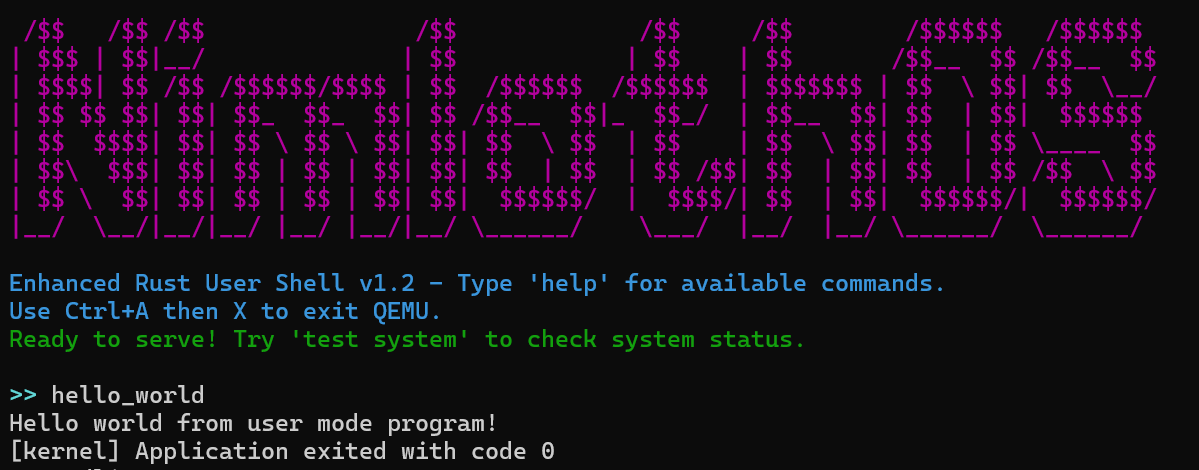
\includegraphics[width=0.5\textwidth]{../image/init_and_helloworld.png}
    \caption{initproc和hello\_world的运行结果}
    \label{fig:init_and_helloworld}
\end{figure}

\begin{figure}[htbp]
    \centering
    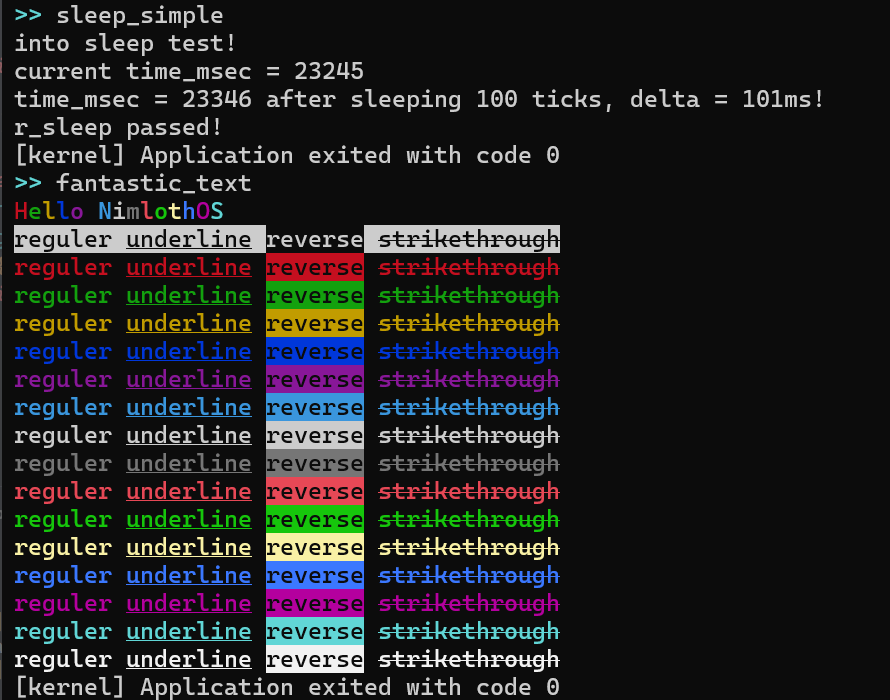
\includegraphics[width=0.5\textwidth]{../image/sleep_test_and_color.png}
    \caption{sleep\_test和fantastic\_text的运行结果}
    \label{fig:sleep_test_and_color}
\end{figure}

\begin{figure}[H]
    \centering
    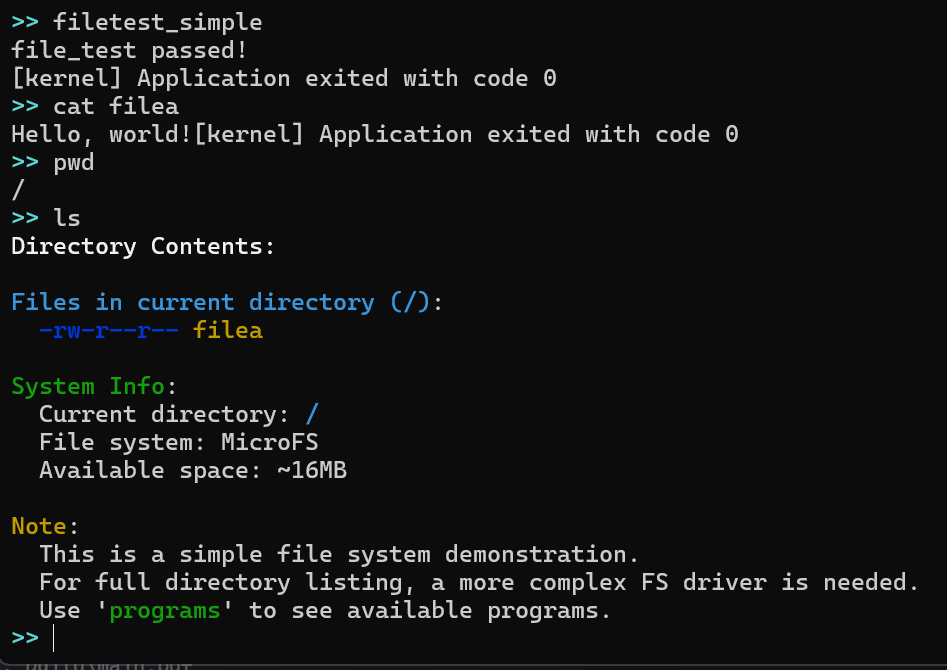
\includegraphics[width=0.5\textwidth]{../image/file.png}
    \caption{文件系统相关}
    \label{fig:file}
\end{figure}

\begin{figure}[htbp]
    \centering
    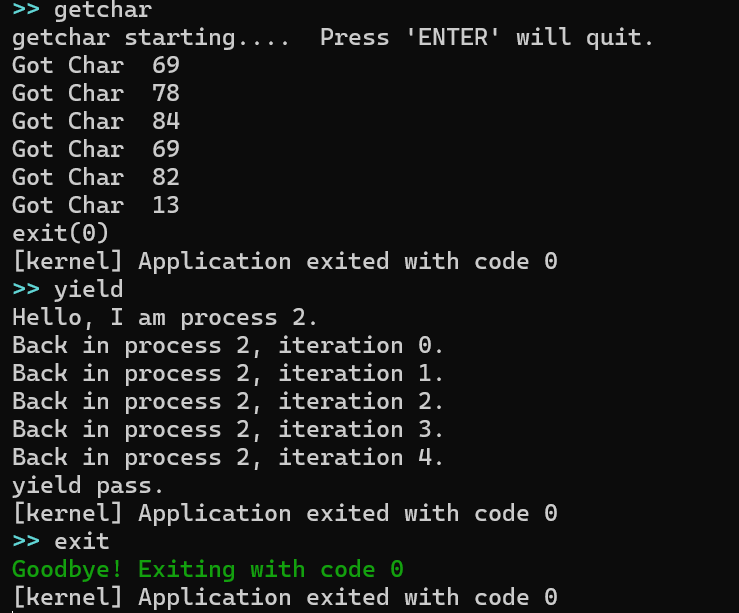
\includegraphics[width=0.5\textwidth]{../image/getchar_yield_exit.png}
    \caption{getchar、yield和exit的运行结果}
    \label{fig:getchar_yield_exit}
\end{figure}

\begin{figure}[htbp]
    \centering
    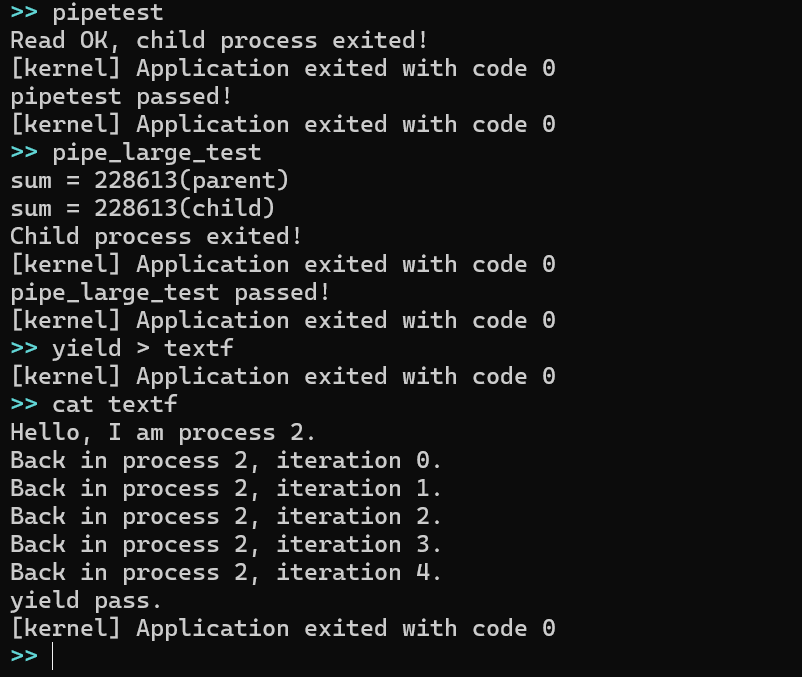
\includegraphics[width=0.5\textwidth]{../image/pipe.png}
    \caption{管道与重定向相关}
    \label{fig:pipe}
\end{figure}

\begin{figure}[htbp]
    \centering
    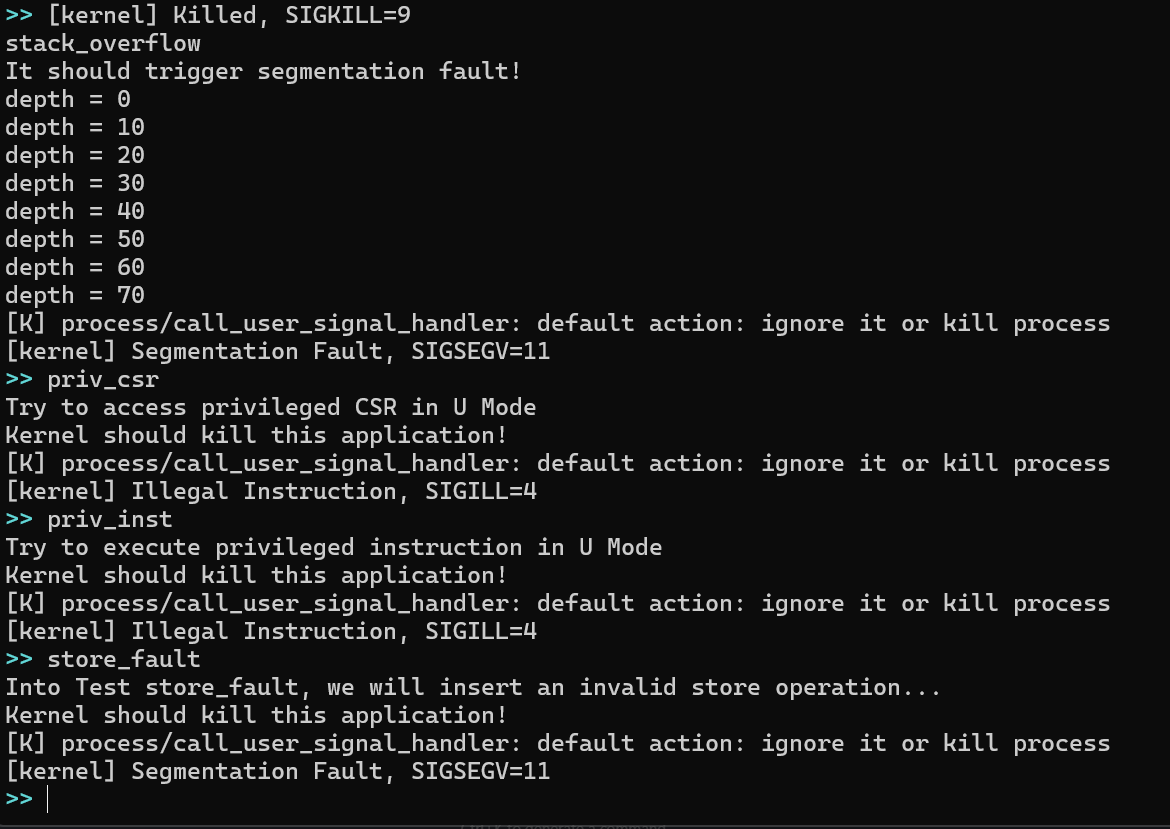
\includegraphics[width=0.5\textwidth]{../image/wrong.png}
    \caption{错误处理测试}
    \label{fig:wrong}
\end{figure}

\begin{figure}[htbp]
    \centering
    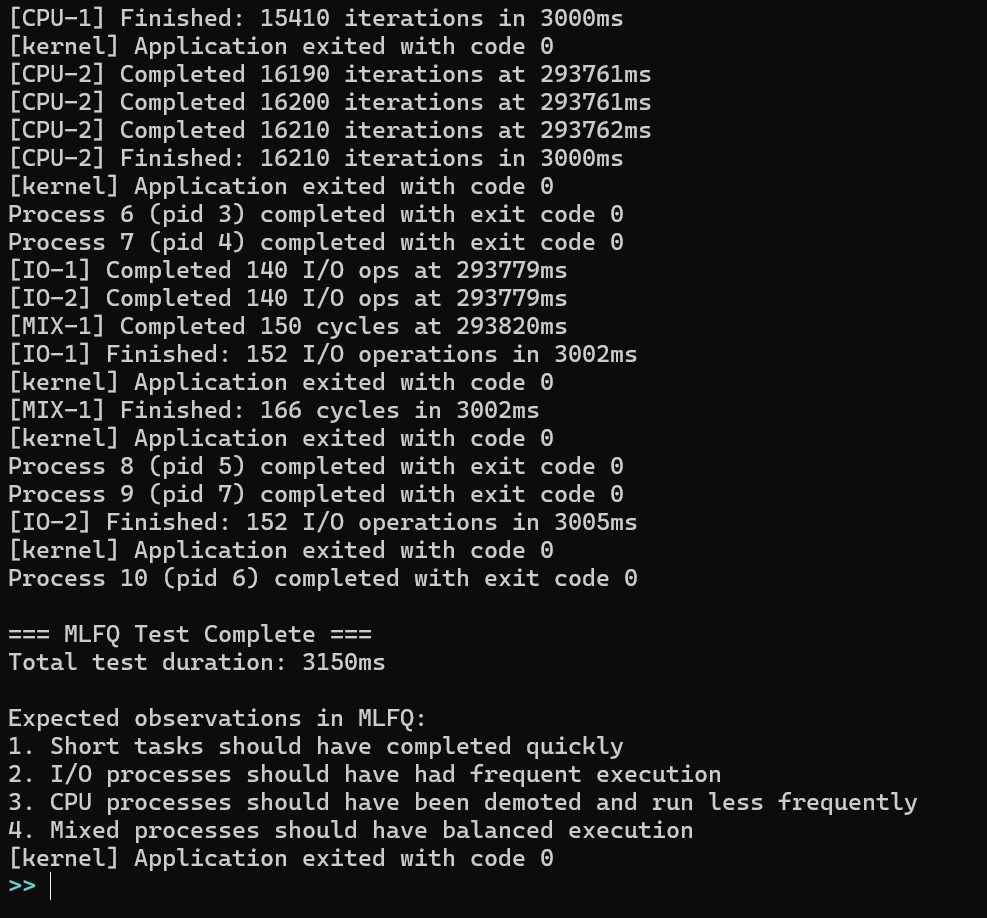
\includegraphics[width=0.5\textwidth]{../image/mlfq.png}
    \caption{MLFQ调度测试}
    \label{fig:mlfq}
\end{figure}

\begin{figure}[htbp]
    \centering
    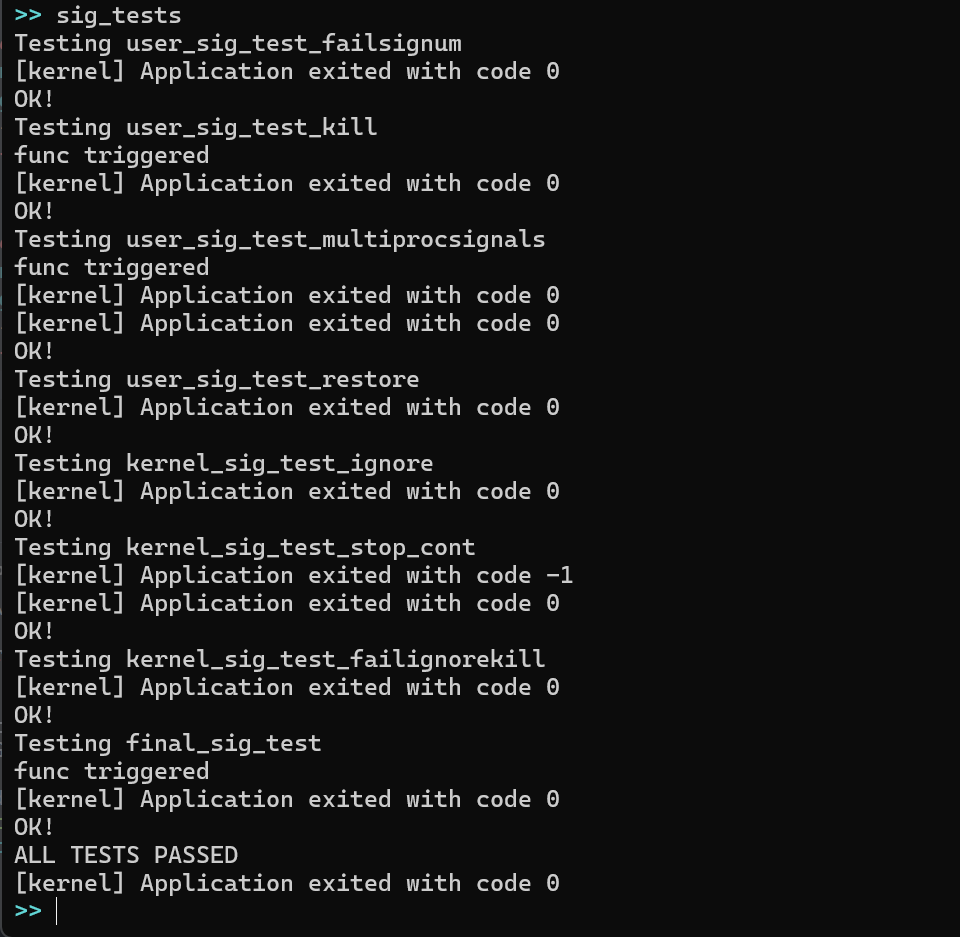
\includegraphics[width=0.5\textwidth]{../image/sig.png}
    \caption{信号处理测试}
    \label{fig:sig}
\end{figure}